\documentclass[aspectratio=169, xcolor={usenames,svgnames,dvipsnames}]{beamer}
\usepackage[utf8]{inputenc}
\usepackage[T1]{fontenc}
\usepackage{graphicx}
\usepackage{grffile}
\usepackage{longtable}
\usepackage{wrapfig}
\usepackage{rotating}
\usepackage[normalem]{ulem}
\usepackage{amsmath}
\usepackage{textcomp}
\usepackage{amssymb}
\usepackage{capt-of}
\usepackage{hyperref}
\usepackage{color}
\usepackage{listings}
\usepackage{mathpazo}
\usepackage{gensymb}
\usepackage{amsmath}
\usepackage{diffcoeff}
\usepackage{steinmetz}
\usepackage{mathtools}
\bibliographystyle{plain}
\usepackage{siunitx}
\sisetup{output-decimal-marker={,}, retain-unity-mantissa = false}
\DeclareSIUnit{\watthour}{Wh}
\hypersetup{colorlinks=true, linkcolor=Blue, urlcolor=Blue}
\renewcommand{\thefootnote}{\fnsymbol{footnote}}
\newcommand{\laplace}[1]{\mathbf{#1}(\mathbf{s})}
\newcommand{\slp}{\mathbf{s}}
\newcommand{\fasor}[1]{\mathbf{#1}(\omega)}
\newcommand{\atan}{\mathrm{atan}}
\parskip=5pt
\usetheme{Boadilla}
\usecolortheme{rose}
\usefonttheme{serif}
\author{Ana Fernández-Guillamón}
\date{}
\title{Fundamentos. Circuitos de Corriente Continua}
\subtitle{Teoría de Circuitos}
\setbeamercolor{alerted text}{fg=blue!50!black} \setbeamerfont{alerted text}{series=\bfseries}
\makeatletter
\patchcmd{\beamer@sectionintoc}{\vskip1.5em}{\vskip1em}{}{}
\makeatother
\AtBeginSubsection[]{\begin{frame}[plain]\tableofcontents[currentsubsection,sectionstyle=show/shaded,subsectionstyle=show/shaded/hide]\end{frame}}
\AtBeginSection[]{\begin{frame}[plain]\tableofcontents[currentsection,hideallsubsections]\end{frame}}
\beamertemplatenavigationsymbolsempty
\setbeamertemplate{footline}[frame number]
\setbeamertemplate{itemize items}[triangle]
\setbeamertemplate{enumerate items}[circle]
\setbeamertemplate{section in toc}[circle]
\setbeamertemplate{subsection in toc}[circle]
\setbeamertemplate{blocks}[shadow=false]

\begin{document}

\maketitle

\section{Introducción}

\begin{frame}{¿Qué es la electricidad?}
\begin{minipage}[c]{0.55\linewidth}
    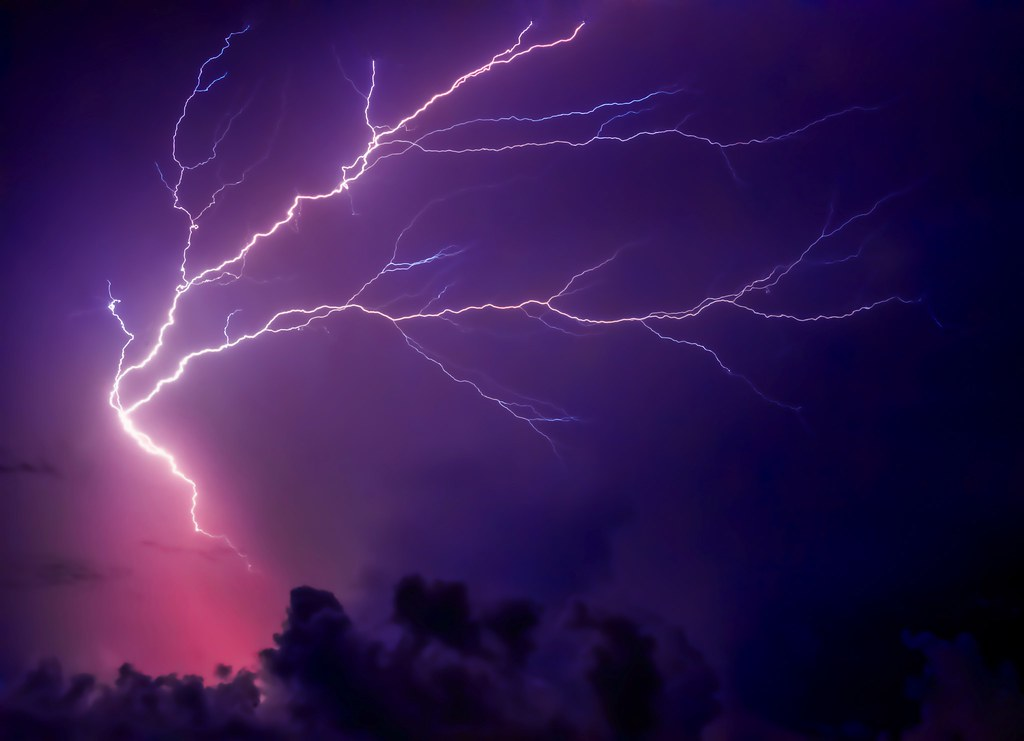
\includegraphics[width=\linewidth]{../figs/26261784989_0c084cd428_b.jpg}
\end{minipage}
\hfill%
\begin{minipage}[c]{0.38\linewidth}
    \pause
    \begin{itemize}
        \item Forma de energía
        \item Prácticamente todas las actividades dependen de ella
        \item Efectos luminosos, mecánicos, caloríficos, etc.
        \item Movimiento de electrones de los átomos
    \end{itemize}
\end{minipage}
\end{frame}

\section{Conceptos fundamentales}

\subsection{Circuito eléctrico}

\begin{frame}{Circuito eléctrico}
\begin{minipage}[c]{0.58\linewidth}
    Un \alert{circuito eléctrico} es un conjunto de componentes eléctricos combinados que crean un camino cerrado por el que puede circular corriente eléctrica. Incluye: 
\begin{itemize}
\item \alert{Elementos activos} (generadores): motivan la circulación de corriente
\item \alert{Elementos pasivos} (receptores): transforman o almacenan la energía eléctrica
\end{itemize}
\end{minipage}
\hfill%
\begin{minipage}[c]{0.3\linewidth}
    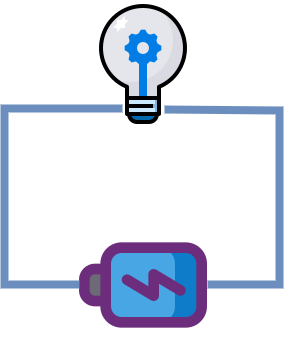
\includegraphics[width=\linewidth]{../figs/circuito.png}
\end{minipage}

\end{frame}

\begin{frame}{Análisis VS. Diseño}
El \alert{análisis} (o resolución) de un circuito eléctrico existente persigue determinar sus condiciones de funcionamiento:
\begin{enumerate}
\item Definir las ecuaciones correspondientes al circuito
\item Obtener los valores de determinadas variables importantes a partir de dichas ecuaciones
\end{enumerate}

El \alert{diseño} (o síntesis) de un circuito eléctrico tiene como objetivo definir el circuito eléctrico, es decir, determinar los componentes necesarios y su interconexión, para obtener unas condiciones de funcionamiento
\end{frame}
% \begin{frame}{Sistemas lineales de parámetros concentrados}
% Todos los circuitos eléctricos que se estudian en esta asignatura se comportan como \alert{sistemas lineales de parámetros concentrados}: 

% \begin{itemize}
% \item \(f(x + y) = f(x) + f(y)\)

% La respuesta \(f\) a la suma de dos entradas \(x\) e \(y\) es igual a la suma de la respuesta individual a cada una de las entradas
% \item \(f(k \cdot x) = k \cdot f(x)\)

% La respuesta a una entrada que está multiplicada por un factor de escala \(k\) es igual a multiplicar por este factor a la respuesta a la entrada.
% \end{itemize}
% \end{frame}

% \begin{frame}[label={sec:org8417777}]{La linealidad es una aproximación de la realidad}
% \begin{itemize}
% \item Estas propiedades simplifican el tratamiento de los circuitos, y \alert{permiten aplicar técnicas de resolución de ecuaciones lineales}.
% \item La linealidad es una \alert{aproximación de la realidad} que no puede aplicarse de manera indiscriminada a cualquier componente y en cualquier condición.
% \item En particular, los \alert{dispositivos electrónicos} como diodos o transistores tienen un \alert{comportamiento} marcadamente \alert{no lineal}, de forma que los circuitos que los contienen no pueden analizarse directamente con las técnicas que aquí se exponen sin realizar previamente aproximaciones de su funcionamiento.
% \end{itemize}
% \end{frame}

% \begin{frame}[label={sec:org0ebbd2c}]{Parámetros concentrados}
% \begin{itemize}
% \item Los circuitos eléctricos reales ocupan espacio, las máquinas generadoras y los receptores tienen grandes dimensiones, y los cables conductores se extienden a lo largo de longitudes variopintas.
% \item Sin embargo, el análisis de circuitos no toma en consideración las propiedades espaciales de los circuitos ni de sus componentes, sino que los confina a elementos puntuales con un modelo de \alert{parámetros concentrados}.
% \item Por ejemplo, un conductor real de \(\SI{100}{\meter}\) se representará habitualmente como un conductor ideal con una resistencia en su punto medio.
% \end{itemize}
% \end{frame}
% \begin{frame}[label={sec:org750a459}]{Simplificación de las ecuaciones de Maxwell}
% \begin{itemize}
% \item Este tratamiento es una simplificación de las ecuaciones del electromagnetismo de Maxwell
% \item Es aplicable únicamente cuando las dimensiones del circuito real son inferiores a la longitud de onda de la señal que circula por el circuito.
% \item Por ejemplo:
% \begin{itemize}
% \item A la frecuencia de \(\SI{50}{\hertz}\), habitual en sistemas eléctricos industriales, la longitud de onda de la señal es de \(\SI{6000}{\kilo\meter}\).
% \item A la frecuencia de \(\SI{2.6}{\giga\hertz}\), característica de la telefonía 4G, la longitud de onda se reduce a \(\SI{11.5}{\centi\meter}\).
% \end{itemize}
% \end{itemize}
% \end{frame}


\subsection{Variables}

\begin{frame}{Variables}
    Las principales \alert{variables} con las que se trabaja en los circuitos eléctricos son:
    \begin{minipage}[c]{0.55\linewidth}
        \begin{itemize}
        \item Corriente eléctrica
        \item Tensión eléctrica
        \item Potencia eléctrica
        \item Energía eléctrica
    \end{itemize}
    \end{minipage}
    \hfill
    \begin{minipage}[c]{0.4\linewidth}
        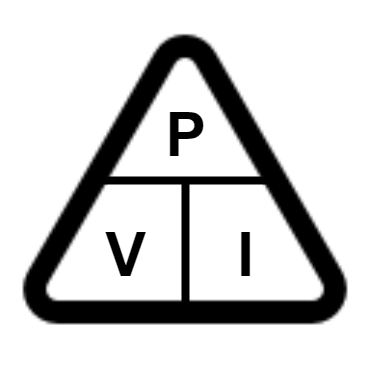
\includegraphics[width=0.6\linewidth]{../figs/piv.jpg}
    \end{minipage}
\end{frame}

\begin{frame}{Corriente eléctrica}{y densidad de corriente}
La \alert{intensidad de la corriente eléctrica} es la variación de la carga \(q(t)\) que atraviesa la sección transversal de un conductor por unidad de tiempo:
\begin{minipage}[c]{0.48\linewidth}
\begin{equation*}
  i(t)=\frac{dq(t)}{dt}
\end{equation*}
\end{minipage}
\hfill
\begin{minipage}[c]{0.48\linewidth}
\begin{center}
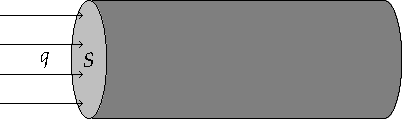
\includegraphics[width=0.8\linewidth]{../figs/seccion_conductor.pdf}
\end{center}
\end{minipage}

Se produce por el \alert{movimiento de electrones} (de $-$ a $+$). Sin embargo, por convenio se considera el \alert{movimiento de cargas positivas} (de $+$ a $-$)

La \alert{unidad} de la corriente es el \alert{amperio} [A]

En ocasiones se habla de \alert{densidad de corriente}:
\begin{equation*}
    \delta=\dfrac{i(t)}{S}
\end{equation*}
\end{frame}

\begin{frame}{Tipos de corriente}{Corriente Continua (CC) y Corriente Alterna (CA)}
\begin{itemize}
\item Corriente continua: siempre fluye en el mismo sentido ($+$ o $-$)
\begin{itemize}
    \item \alert{CC constante} $\equiv$ corriente continua
    \item CC variable
\end{itemize}
\item Corriente alterna: cambia de sentido cada cierto tiempo
\begin{itemize}
    \item \alert{CA sinusoidal} $\equiv$ corriente alterna
    \item CA periódica
    \item CA aperiódica
\end{itemize}
\end{itemize}
\end{frame}

\begin{frame}{Tipos de corriente}{Corriente Continua (CC) y Corriente Alterna (CA)}
\begin{itemize}
\item Corriente Continua (\(\frac{d}{dt} = 0\))
\end{itemize}
\begin{center}
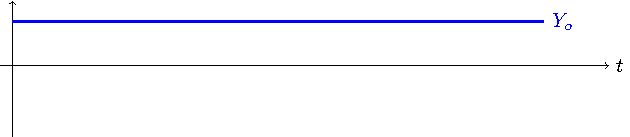
\includegraphics[height=0.25\textheight]{../figs/continua.pdf}
\end{center}

\begin{itemize}
\item Corriente Alterna (\(\frac{d}{dt} \neq 0\))
\end{itemize}
\begin{center}
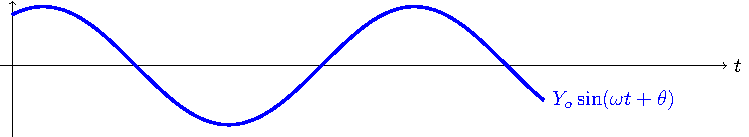
\includegraphics[height=0.25\textheight]{../figs/sin.pdf}
\end{center}
\end{frame}

\begin{frame}{Tensión eléctrica y f.e.m.}
El \alert{potencial eléctrico en un punto}, \(v(t)\),  es la energía potencial que tiene una carga unitaria en ese punto debida al campo eléctrico

La \alert{tensión} o \alert{diferencia de potencial entre dos puntos} A y B, \(u_{AB}(t)\), es el trabajo realizado por el campo eléctrico al desplazar una carga unitaria entre esos puntos

\begin{minipage}[c]{0.5\linewidth}
\begin{equation*}
  u_{AB}(t) = v_A(t) - v_B(t) = \frac{dW_{e}}{dq}
\end{equation*}
\end{minipage}
\hfill
\begin{minipage}[c]{0.4\linewidth}
\begin{center}
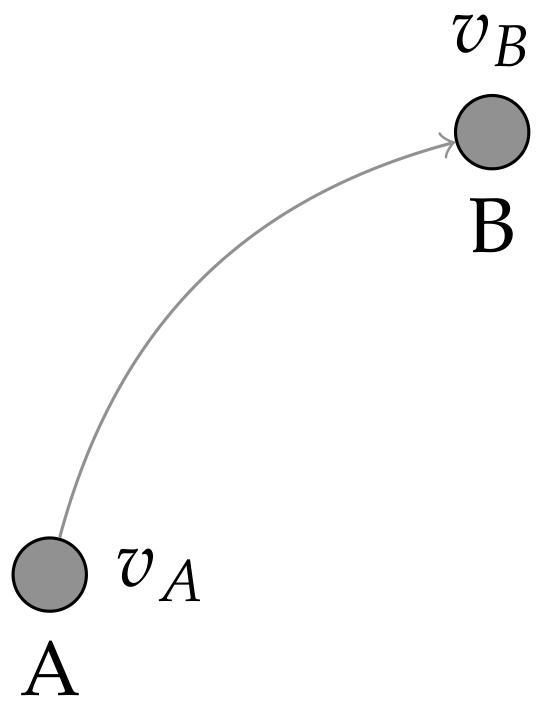
\includegraphics[height=0.3\textheight]{../figs/tension_puntos.PNG}
\end{center}
\end{minipage}

La \alert{fuerza electromotriz} (f.e.m.) es la causa que mantiene a los electrones en movimiento (energía cedida por unidad de carga), y la proporcionan los elementos activos (\alert{generadores})

La \alert{unidad} de todas estas magnitudes es el \alert{voltio} [V]
\end{frame}

\begin{frame}{La trayectoria no importa, pero el signo depende del sentido}
\begin{minipage}[c]{0.5\linewidth}
    \begin{itemize}
    \item $u_{AB}(t)$ \alert{no depende de la trayectoria} del desplazamiento, sino solo del potencial en cada punto $\rightarrow$ \alert{campo conservativo}
    \item Aunque la trayectoria no sea relevante, hay que tener en cuenta el \alert{sentido del desplazamiento}
\end{itemize}
\end{minipage}
\hfill
\begin{minipage}[c]{0.45\linewidth}
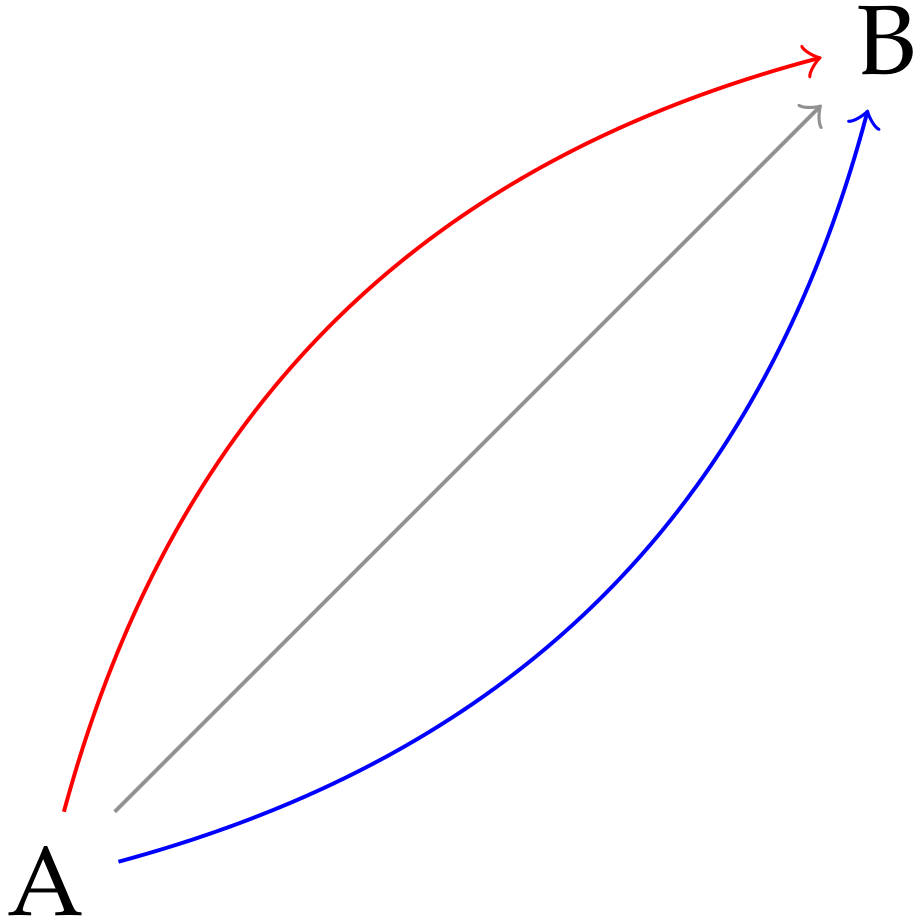
\includegraphics[width=0.45\linewidth]{../figs/diagrama_tension.PNG}
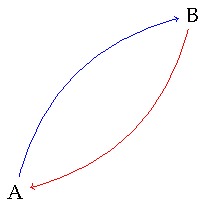
\includegraphics[width=0.45\linewidth]{../figs/sentido_tension.pdf}
\end{minipage}

Si el movimiento se produce desde B hasta A, el signo es contrario al anterior:

\begin{equation*}
  u_{BA} = v_B - v_A = - u_{AB} 
\end{equation*}
\end{frame}

\begin{frame}{Potencia eléctrica}
La \alert{potencia eléctrica} es la variación del trabajo del campo eléctrico por unidad de tiempo:

\begin{equation*}
  p(t)=\frac{dW_{e}}{dt}= \underbrace{\dfrac{dW_e}{dq(t)}}_{u(t)} \cdot \underbrace{\dfrac{dq(t)}{dt}}_{i(t)}
\end{equation*}

La \alert{unidad} de la potencia eléctrica es el \alert{vatio} [W]
\end{frame}

\begin{frame}{Potencia eléctrica}{Convenio de signos -- Receptores y generadores}
Para determinar el \alert{signo de la potencia eléctrica} hay que tener en consideración los signos de las variables de las que depende, la tensión y la corriente. 
\begin{itemize}
\item Flechas en \alert{mismo sentido}: potencia \alert{positiva} (absorbe potencia) $\rightarrow$ \alert{receptor}
\begin{itemize}
    \item La corriente \emph{entra} por el terminal de mayor potencial
\end{itemize}
\item Flechas en \alert{sentidos opuestos}: potencia \alert{negativa} (genera potencia) $\rightarrow$ \alert{generador}
\begin{itemize}
    \item La corriente \emph{sale} por el terminal de mayor potencial
\end{itemize}
\end{itemize}

\begin{center}
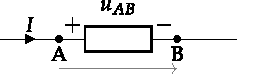
\includegraphics[height=0.17\textheight]{../figs/signo_potencia1.pdf}
\hfil
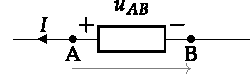
\includegraphics[height=0.17\textheight]{../figs/signo_potencia2.pdf}
\end{center}
\end{frame}

\begin{frame}{Potencia y Energía}
\begin{description}
\item[{Potencia}] Cantidad de trabajo realizado por unidad de tiempo
\begin{description}
\item[{Unidades}] [W], [kW]
\end{description}
\item[{Energía}] Capacidad para realizar un trabajo: $E=P\cdot t$
\begin{description}
\item[{Unidades}] [J], [Wh], [kWh]
\end{description}
\end{description}
\end{frame}





\section{Leyes básicas}

\subsection{Ley de Ohm}

\begin{frame}{Ley de Ohm}
\begin{columns}
\begin{column}{0.4\linewidth}
Relación \alert{lineal} entre tensión e intensidad: \[
\boxed{u(t) = R \cdot i(t)}
\]
\end{column}
\begin{column}{0.6\linewidth}
\begin{center}
    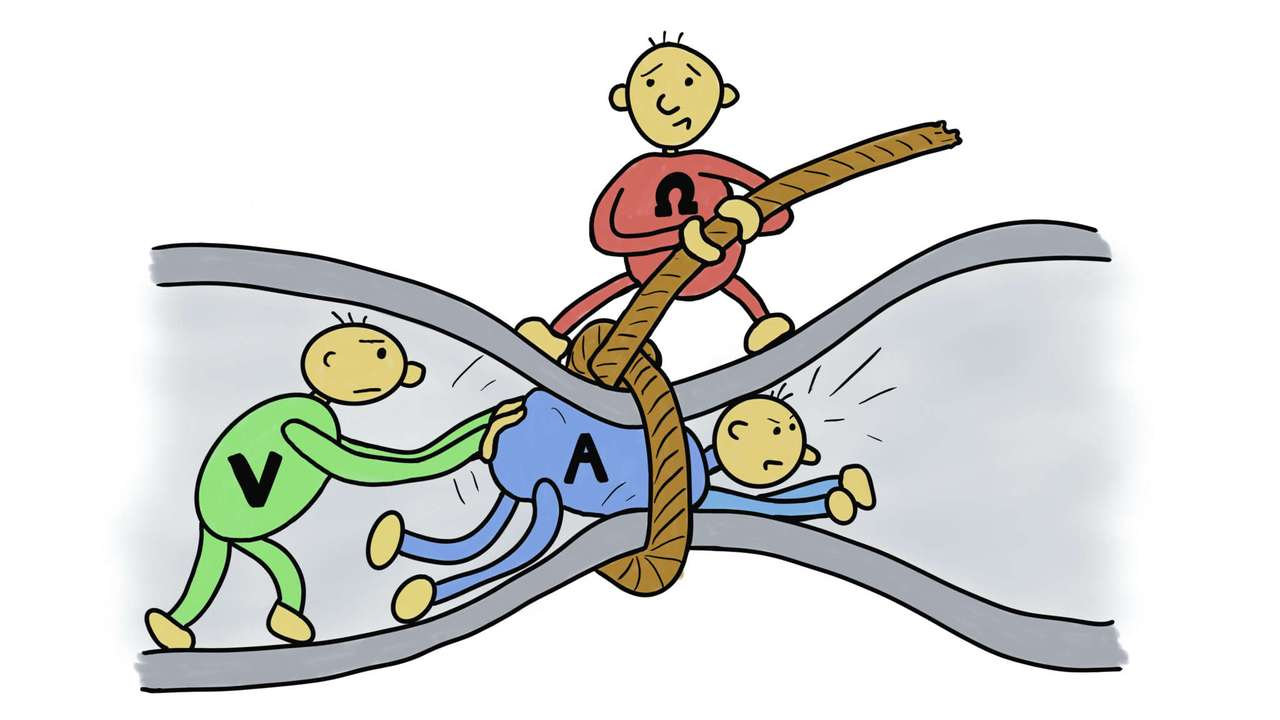
\includegraphics[width=\linewidth]{../figs/ohm.jpg}
\end{center}
\end{column}
\end{columns}
    
\end{frame}

\subsection{Leyes de Kirchhoff}

\begin{frame}{Definiciones}
\begin{description}
\item[{Nudo}] unión de \alert{3} o más conductores
\item[{Rama}] elementos conectados entre dos nudos consecutivos
\item[{Lazo}] conjunto de ramas que forman un camino cerrado
\item[{Malla}] lazo que no contiene ningún otro en su interior
\end{description}

\begin{center}
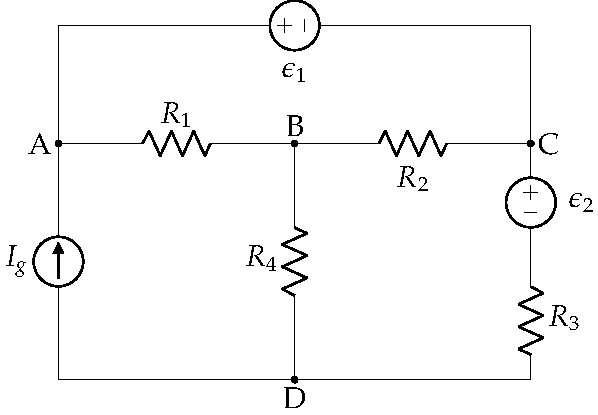
\includegraphics[height=0.5\textheight]{../figs/mallas.pdf}
\end{center}
\end{frame}

\begin{frame}{Primera Ley de Kirchhoff (1LK)}
\begin{itemize}
\item La \alert{1LK} es el principio de conservación de la carga aplicado a los circuitos eléctricos

\item \alert{LKC}: la suma de las corrientes que llegan a un nudo es igual a la suma de las que salen:
\begin{equation*}
			\boxed{\sum_{i=1}^n i_i(t)=0}
		\end{equation*}
\end{itemize}
\begin{center}
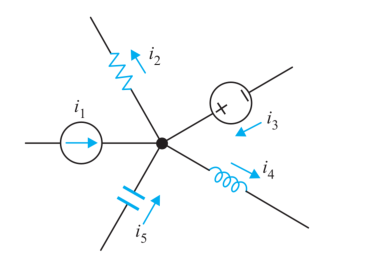
\includegraphics[height=0.4\textheight]{../figs/LKC_FM.pdf}
\end{center}
\end{frame}

\begin{frame}{Segunda Ley de Kirchhoff (2LK)}
\begin{itemize}
\item La \alert{2LK} es el principio de conservación de la energía aplicado a los circuitos eléctricos

\item \alert{LKV}: la suma (con signo) de las tensiones a lo largo de un camino cerrado es cero:
\begin{equation*}
			\boxed{\sum_{j=1}^m u_i(t)=0}
		\end{equation*}

\begin{itemize}
\item La energía producida por un generador es consumida por los receptores del circuito para producir trabajo (mecánico, químico, etc.) o calor.
\end{itemize}
\end{itemize}

\begin{center}
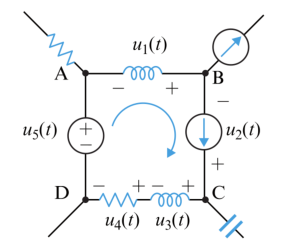
\includegraphics[height=0.35\textheight]{../figs/LKV_FM.pdf}
\end{center}
\end{frame}

\section{Elementos de los circuitos}

\subsection{Elementos activos}
\label{sec:org2b18ef6}

\begin{frame}{Generadores de tensión}
Proporcionan una diferencia de potencial $U$ entre sus bornes de salida (\alert{impone la tensión})
\begin{columns}
\begin{column}{0.3\columnwidth}
\begin{center}
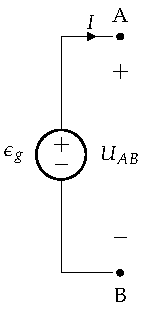
\includegraphics[height=0.5\textheight]{../figs/FuenteTensionIdealDC.pdf}

\alert{Ideal}
\begin{equation*}
    u_{AB}=\epsilon_g
\end{equation*}
\end{center}
\end{column}
\begin{column}{0.3\columnwidth}
\begin{center}
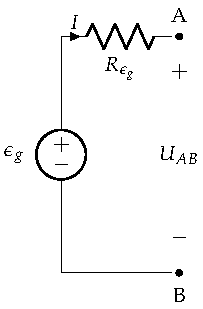
\includegraphics[height=0.5\textheight]{../figs/FuenteTensionRealDC.pdf}

\alert{Real} (pérdidas)
\begin{equation*}
    u_{AB}<\epsilon_g
\end{equation*}
\end{center}
\end{column}
\begin{column}{0.4\columnwidth}
\begin{align*}
    P_g&=\epsilon_g\cdot I\\
    P_p&=R_{\epsilon_g}\cdot I^2\\
    P_u&=U_{AB}\cdot I\\
    \Aboxed{\epsilon_g&=U_{AB}+R_{\epsilon_g}\cdot I}
\end{align*}
\end{column}
\end{columns}
\end{frame}

\begin{frame}{Generadores de corriente}
Proporcionan una corriente $I$ (\alert{impone la corriente})
\begin{columns}
\begin{column}{0.3\columnwidth}
\begin{center}
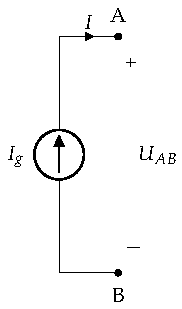
\includegraphics[height=0.5\textheight]{../figs/FuenteCorrienteIdeal.pdf}

\alert{Ideal}
\begin{equation*}
    I=I_g
\end{equation*}
\end{center}
\end{column}
\begin{column}{0.3\columnwidth}
\begin{center}
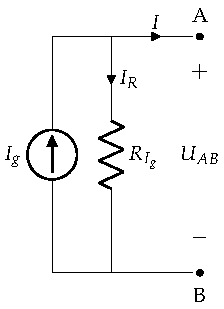
\includegraphics[height=0.5\textheight]{../figs/FuenteCorrienteRealDC.pdf}

\alert{Real} (pérdidas)
\begin{equation*}
    I<I_g
\end{equation*}
\end{center}
\end{column}
\begin{column}{0.4\columnwidth}
\begin{align*}
    P_g&=U_{AB}\cdot I_g\\
    P_p&=\dfrac{U_{AB}^2}{R_{I_g}}\\
    P_u&=U_{AB}\cdot I\\
    \Aboxed{I_g&=I+\dfrac{U_{AB}}{R_{I_g}}}
\end{align*}
\end{column}
\end{columns}
\end{frame}

\begin{frame}{Dualidad de generadores}
    Dos fuentes son equivalentes cuando suministran el \alert{mismo valor de tensión y corriente} a un circuito externo (solo puede darse entre \alert{fuentes reales})
    \begin{columns}
\begin{column}{0.3\columnwidth}
\begin{center}
\vspace{-8mm}
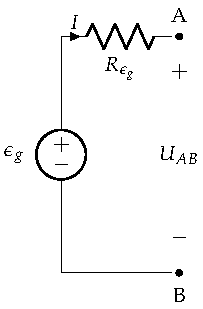
\includegraphics[height=0.4\textheight]{../figs/FuenteTensionRealDC.pdf}\\
\begin{equation*}
		U_{AB} = \epsilon_g - R_{\epsilon_g} \cdot I
	\end{equation*}
\end{center}
\end{column}
\begin{column}{0.3\columnwidth}
\begin{center}
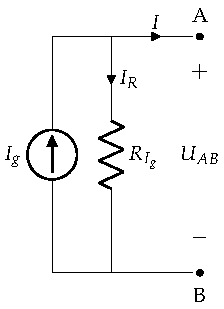
\includegraphics[height=0.4\textheight]{../figs/FuenteCorrienteRealDC.pdf}\\
\begin{align*}
		I &= I_g - \frac{U_{AB}}{R_{I_g}} \\
		U_{AB} &= R_{I_g} \cdot I_g - R_{I_g} \cdot I
	\end{align*} 
\end{center}
\end{column}
\begin{column}{0.4\columnwidth}
\begin{center}
    Si $R_g = R_{\epsilon_g} = R_{I_g}$:
	\begin{equation*}
		\boxed{\epsilon_g = R_{g} \cdot I_g \Leftrightarrow {I_g = \frac{\epsilon_g}{R_g}}}  
	\end{equation*}
	
	\alert{El polo $+$ queda en la misma posición que la flecha}
\end{center}
\end{column}
\end{columns}
\end{frame}

\begin{frame}{Dualidad de generadores}{Ejemplo}
Convertir en fuente de tensión o intensidad, según corresponda
    \begin{center}
	        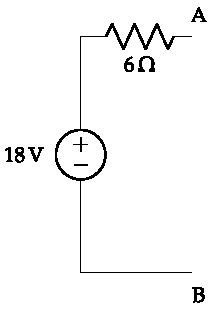
\includegraphics[height=3.7cm]{../figs/Conversion_Fuentes.pdf}\hfil
	        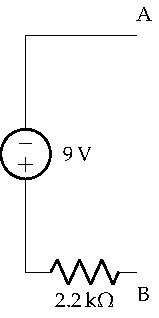
\includegraphics[height=3.7cm]{../figs/Conversion_Fuentes_2.pdf}\hfil
	        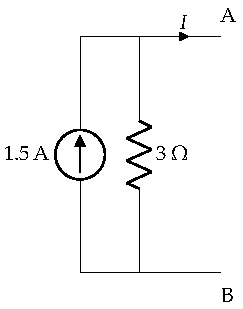
\includegraphics[height=3.7cm]{../figs/Conversion_Fuentes_3.pdf}\hfil
	        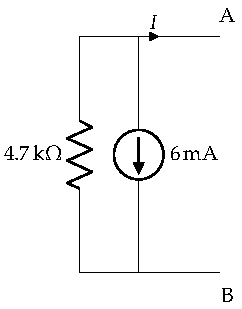
\includegraphics[height=3.7cm]{../figs/Conversion_Fuentes_4.pdf}
	    \end{center}
\end{frame}

\begin{frame}{Generadores dependientes}
    No tienen valores de $\epsilon$ o $i_g$ fijos, sino que \alert{dependen de la tensión o corriente en otros puntos de la red}:
	\begin{center}
		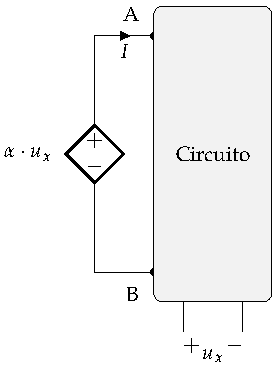
\includegraphics[height=4cm]{../figs/FuenteTensionDependienteTension.pdf}\label{fig.tension-tension}\hfill
		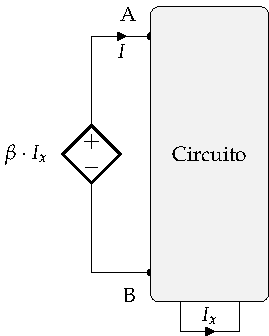
\includegraphics[height=4cm]{../figs/FuenteTensionDependienteCorriente.pdf}\label{fig.tension-corriente}\hfill
		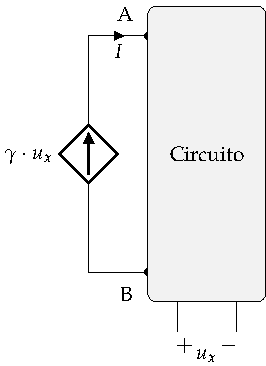
\includegraphics[height=4cm]{../figs/FuenteCorrienteDependienteTension.pdf}\label{fig.corriente-tension}\hfill
		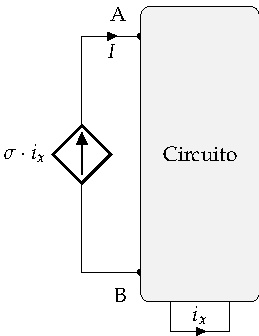
\includegraphics[height=4cm]{../figs/FuenteCorrienteDependienteCorriente.pdf}\label{fig.corriente-corriente}
	\end{center}
\end{frame}

\subsection{Elementos pasivos}
\begin{frame}{Resistencia}
\begin{itemize}
\item Una \alert{resistencia} $R$ provoca una \alert{diferencia de potencial} entre sus terminales \alert{directamente proporcional} a su corriente:  [\(\Omega\)]
\[
\boxed{u(t) = R \cdot i(t)}
\]
\item \alert{Criterio de signos}: la tensión es positiva en el terminal por el que entra la corriente (las flechas de tensión y corriente tienen el mismo sentido)
\end{itemize}
\begin{columns}
\begin{column}{0.5\columnwidth}
\begin{center}
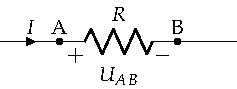
\includegraphics[height=0.2\textheight]{../figs/Resistencia.pdf}
\end{center}
\end{column}
\begin{column}{0.5\columnwidth}
\begin{center}
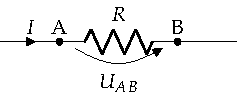
\includegraphics[height=0.2\textheight]{../figs/Resistencia_Flecha.pdf}
\end{center}
\end{column}
\end{columns}
\end{frame}

\begin{frame}{Resistencia}{Resistividad}
La \alert{resistividad} del material determina si éste es mejor o peor conductor (depende de $T$)
\begin{equation*}
  R = \rho \cdot \frac{l}{S}
\end{equation*}

\begin{itemize}
\item La \alert{sección} se expresa en \(\si{\milli\meter\squared}\)

\item La \alert{resistividad} depende del material conductor y de la temperatura ambiente:
\begin{itemize}
\item Cobre a 20ºC: \(\qty[parse-numbers = false]{1/58}{\ohm\milli\meter\squared/\meter}\)
\item Aluminio a 20ºC: \(\qty[parse-numbers = false]{1/36}{\ohm\milli\meter\squared/\meter}\)
\end{itemize}
\end{itemize}
\begin{minipage}[c]{0.48\linewidth}
Para otras temperaturas:
\begin{align*}
    \rho_f&=\rho_{20}\cdot (1+\alpha\cdot (T_f-20)) \\
	R_f&=R_{20}\cdot (1+\alpha\cdot (T_f-20))
\end{align*}
\end{minipage}
\hfill
\begin{minipage}[c]{0.48\linewidth}
$\alpha \equiv$ coeficiente de temperatura
\end{minipage}
\end{frame}

\begin{frame}{Conductancia}{Conductividad}
    	La inversa de la resistencia es la \alert{conductancia} [S]: facilidad de los conductores al paso de la corriente eléctrica:
	\begin{equation*}
		\boxed{G=\dfrac{1}{R}}
	\end{equation*}
	
	La inversa de la resistividad es la \alert{conductividad} [m$/\Omega$ mm$^2$]: facilidad de los materiales al paso de la corriente:
	\begin{equation*}
		\gamma=\dfrac{1}{\rho}
	\end{equation*}
\end{frame}

\begin{frame}{Ley de Joule}
\begin{center}
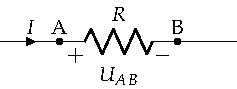
\includegraphics[height=0.2\textheight]{../figs/Resistencia.pdf}
\end{center}

\begin{itemize}
\item \alert{Ley de Joule}: una resistencia disipa energía eléctrica produciendo \alert{calor}
\end{itemize}
\[
\boxed{p(t)=R\cdot i^{2}(t)}
\]
\end{frame}

\begin{frame}{Cortocircuito y Circuito Abierto}
\begin{itemize}
\item Cortocircuito: resistencia nula (tensión nula)
\end{itemize}

\begin{center}
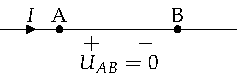
\includegraphics[height=0.2\textheight]{../figs/Cortocircuito.pdf}
\end{center}

\begin{itemize}
\item Circuito abierto: resistencia infinita (corriente nula)
\end{itemize}

\begin{center}
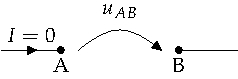
\includegraphics[height=0.2\textheight]{../figs/CircuitoAbierto.pdf}
\end{center}
\end{frame}

\begin{frame}{Bobina o inductancia}

\alert{Bobina:} conductor arrollado alrededor de un núcleo
\begin{center}
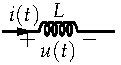
\includegraphics[height=0.2\textheight]{../figs/Bobina.pdf}
\end{center}

La tensión en sus terminales es directamente proporcional al cambio de la corriente: coeficiente de autoinducción o \alert{inductancia} [H]:
\[
u_L(t)=L\cdot\frac{di(t)}{dt}\rightarrow
	i(t_f)=i(t_i)+\dfrac{1}{L}\cdot\int_{t_i}^{t_f} u(t)\cdot dt
\]

La inductancia $L$ expresa la relación entre el cambio de flujo y el cambio de corriente:
\begin{equation*}
		L= \dfrac{d\phi(t)}{di(t)}
	\end{equation*}


\end{frame}

\begin{frame}[label={sec:org8fdbc9a}]{Bobina o inductancia}
\begin{center}
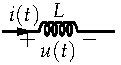
\includegraphics[height=0.2\textheight]{../figs/Bobina.pdf}
\end{center}

\begin{itemize}
\item Almacena \alert{energía magnética}:
\end{itemize}
\[
  E_L(t) = \int_{-\infty}^t u(\tau) \cdot i(\tau) d\tau = \frac{1}{2} \cdot L \cdot i^2(t)
\]
\begin{itemize}
\item En circuitos de CC es un \alert{cortocircuito}:
\end{itemize}
\begin{equation*}
  \frac{di(t)}{dt} = 0 \Rightarrow U_L = 0
\end{equation*}
\end{frame}

\begin{frame}{Condensador}
\alert{Condensador}: dos placas metálicas separadas por una capa dieléctrica. Al aplicar tensión se produce una \alert{separación de cargas opuestas} que se \alert{acumulan} en cada placa
\begin{center}
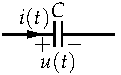
\includegraphics[height=0.2\textheight]{../figs/Condensador.pdf}
\end{center}

\begin{itemize}
\item La \alert{carga acumulada} en un instante es \alert{proporcional} a la \alert{diferencia de potencial} en ese instante: \alert{capacidad} [F]
\[
q(t) = C \cdot u(t)
\]
\item En el proceso de carga se produce una corriente eléctrica entre las dos placas:
\end{itemize}
\begin{equation*}
    i_C(t)=\frac{dq(t)}{dt}=C\frac{du(t)}{dt}\rightarrow u(t_f)=u(t_i)+\dfrac{1}{C}\cdot\int_{t_i}^{t_f} i(t)\cdot dt
\end{equation*}

\end{frame}


\begin{frame}{Condensador}
\begin{center}
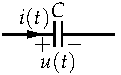
\includegraphics[height=0.2\textheight]{../figs/Condensador.pdf}
\end{center}

\begin{itemize}
\item Un condensador almacena \alert{energía eléctrica}:
\end{itemize}
\[
  E_c(t) = \int_{-\infty}^t u(\tau) \cdot i(\tau) d\tau = \frac{1}{2} \cdot C \cdot u^2(t)
\]

\begin{itemize}
\item En un circuito de corriente continua se comporta como un \alert{circuito abierto}:
\end{itemize}
\begin{equation*}
  \frac{du(t)}{dt} = 0 \Rightarrow I_c = 0
\end{equation*}
\end{frame}

\begin{frame}{Otros receptores}
\begin{itemize}
    \item Compuestos por combinaciones de los elementos básicos
    \item Se caracterizan por su \alert{fuerza contraelectromotriz} (f.c.e.m, E' o $\varepsilon'$): energía por unidad de carga que transforman en otro tipo (no calor)
\end{itemize}
\begin{columns}
\begin{column}{0.3\columnwidth}
\begin{center}
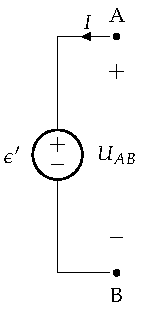
\includegraphics[height=0.4\textheight]{../figs/receptor_ideal.pdf}

\alert{Ideal}
\begin{equation*}
    u_{AB}=\epsilon'
\end{equation*}
\end{center}
\end{column}
\begin{column}{0.3\columnwidth}
\begin{center}
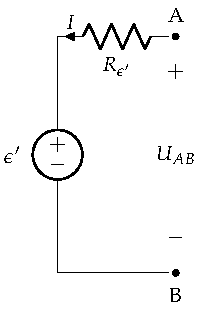
\includegraphics[height=0.4\textheight]{../figs/receptor_real.pdf}

\alert{Real} (pérdidas)
\begin{equation*}
    u_{AB}>\epsilon'
\end{equation*}
\end{center}
\end{column}
\begin{column}{0.4\columnwidth}
\begin{align*}
    P_u&=\epsilon'\cdot I\\
    P_p&=R_{\epsilon'}\cdot I^2\\
    P_a&=U_{AB}\cdot I\\
    \Aboxed{U_{AB}&=\epsilon'+R_{\epsilon'}\cdot I}
\end{align*}
\end{column}
\end{columns}
\end{frame}

\begin{frame}{Eficiencia}

Cociente entre la potencia de salida y la potencia de entrada:
\begin{itemize}
    \item Receptor (generalmente, motor):
\begin{equation*}
  \eta_m = \frac{P_{util}}{P_{absorbida}}
\end{equation*}

\item Generador:
\begin{equation*}
  \eta_g = \frac{P_{entregada}}{P_{producida}}
\end{equation*}
\end{itemize}




Cualquier máquina tiene pérdidas:

\begin{equation*}
  \boxed{\eta < 1}
\end{equation*}
\end{frame}

\begin{frame}{Elementos de los circuitos}{Ejemplo}
Un generador de corriente continua, $fem=\SI{500}{\volt}$ y $\SI{0.75}{\ohm}$ de resistencia, alimenta mediante una línea de cobre de $\SI{18}{\milli\ohm\milli\meter\per\meter}$ y $\SI{16}{\milli\meter\squared}$ de sección a un motor de 1 CV y rendimiento 74.49\%, situado a $\SI{1}{\kilo\meter}$ de distancia. Se pide determinar:
	    \begin{itemize}
	        \item Intensidad de corriente en el motor y densidad de corriente, sabiendo que ésta no debe superar $\SI{2}{\ampere/ \milli\meter\squared}$
	        \item Tensiones en bornes del generador y del motor, así como la caída de tensión en la línea
	        \item $fcem$ del motor y su resistencia
	    \end{itemize}
\end{frame}


\section{Asociación de elementos}

\begin{frame}{Asociación de elementos}
    Las asociaciones principales de los elementos son:
    \begin{itemize}
        \item \alert{Serie}: final con principio $\rightarrow$ misma corriente
        \item \alert{Paralelo}: todos los principios en un punto, todos los finales en otro $\rightarrow$ misma diferencia de potencial
        \item \alert{Mixto}: combinación de serie y paralelo
        \item \alert{Estrella - Triángulo}: conexión de cargas trifásicas
    \end{itemize}
    
\end{frame}


\subsection{Conexión en serie} 

\begin{frame}{Conexión en serie}{Resistencias}
\begin{columns}
\begin{column}{0.3\columnwidth}
\begin{center}
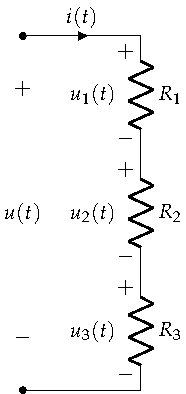
\includegraphics[height=0.85\textheight]{../figs/AsociacionSerie.pdf}
\end{center}
\end{column}
\begin{column}{0.7\columnwidth}
\begin{align*}
  u(t) & = u_1(t) + u_2(t) + u_3(t)\\
  u_1(t) &= R_1 \cdot i(t)\\
  u_2(t) &= R_2 \cdot i(t)\\
  u_3(t) &= R_3 \cdot i(t)\\
  u(t)& = i(t) \cdot (R_1 + R_2 + R_3)\\
  \Aboxed{R_{eq} &= \sum_{i = 1}^n R_i}
\end{align*}
\end{column}
\end{columns}
\end{frame}

\begin{frame}{Conexión en serie}{Divisor de tensión}
\begin{columns}
\begin{column}{0.3\columnwidth}
\begin{center}
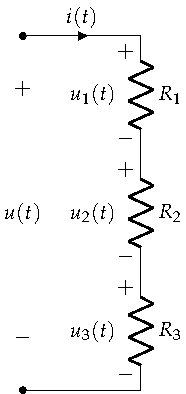
\includegraphics[height=0.85\textheight]{../figs/AsociacionSerie.pdf}
\end{center}
\end{column}
\begin{column}{0.7\columnwidth}
\begin{align*}
  i(t) &= \frac{u(t)}{R_1 + R_2 + R_3}\\
  u_3(t) &= R_3 \cdot i(t)\\ 
  u_3(t) &= u(t) \cdot \frac{R_3}{R_1 + R_2 + R_3}  
\end{align*}

En general:
\begin{equation*}
  \boxed{u_o(t) = u(t) \cdot \frac{R_o}{R_{eq}}}
\end{equation*}
\end{column}
\end{columns}
\end{frame}

\begin{frame}{Conexión en serie}{Bobinas}
\begin{columns}
\begin{column}{0.3\columnwidth}
\begin{center}
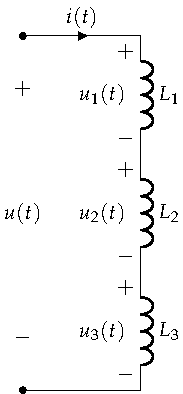
\includegraphics[height=0.85\textheight]{../figs/BobinasSerie.pdf}
\end{center}
\end{column}
\begin{column}{0.7\columnwidth}
\begin{align*}
  u(t) & = u_1(t) + u_2(t) + u_3(t)\\
  u_1(t) &= L_1 \cdot \frac{di(t)}{dt}\\
  u_2(t) &= L_2 \cdot \frac{di(t)}{dt}\\
  u_3(t) &= L_3 \cdot \frac{di(t)}{dt}\\
  u(t)& = \frac{di(t)}{dt} \cdot (L_1 + L_2 + L_3)\\
  \Aboxed{L_{eq} &= \sum_{i = 1}^n L_i}
\end{align*}
\end{column}
\end{columns}
\end{frame}

\begin{frame}{Conexión en serie}{Condensadores}
\begin{columns}
\begin{column}{0.3\columnwidth}
\begin{center}
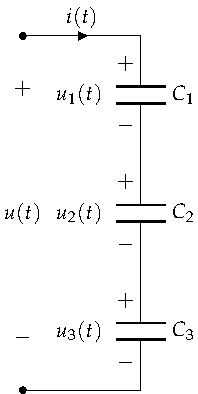
\includegraphics[height=0.85\textheight]{../figs/CondensadoresSerie.pdf}
\end{center}
\end{column}
\begin{column}{0.7\columnwidth}
\begin{align*}
  u(t) & = u_1(t) + u_2(t) + u_3(t)\\
  i(t) &= C_1 \cdot \frac{du_1(t)}{dt}= C_2 \cdot \frac{du_2(t)}{dt}= C_3 \cdot \frac{du_3(t)}{dt}\\
  u_1(t)&=\dfrac{1}{C_1}\cdot\int_{0}^{t} i(t)\, dt\\
  u_2(t)&=\dfrac{1}{C_2}\cdot\int_{0}^{t} i(t)\, dt\\
  u_3(t)&=\dfrac{1}{C_3}\cdot\int_{0}^{t} i(t)\, dt\\
  u(t)& = \int i(t)\,dt \cdot \left(\dfrac{1}{C_1}+\dfrac{1}{C_2}+\dfrac{1}{C_3}\right)\\
  \Aboxed{\frac{1}{C_{eq}} &= \sum_{i = 1}^n \frac{1}{C_i}}
\end{align*}
\end{column}
\end{columns}
\end{frame}

\subsection{Conexión en paralelo}

\begin{frame}{Conexión en paralelo}{Resistencias}
\begin{columns}
\begin{column}{0.4\columnwidth}
\begin{center}
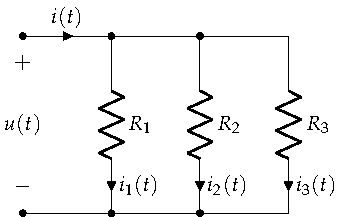
\includegraphics[width=.9\linewidth]{../figs/AsociacionParalelo.pdf}
\end{center}
\end{column}
\begin{column}{0.6\columnwidth}
\begin{align*}
  i(t)& = i_1(t) + i_2(t) + i_3(t)\\
  i_1(t) &= u(t)/R_1\\
  i_2(t) &= u(t)/R_2\\
  i_3(t) &= u(t)/R_3\\
  i(t) &= u(t) \cdot \left(\frac{1}{R_1} + \frac{1}{R_2} + \frac{1}{R_3}\right)\\
  \Aboxed{\frac{1}{R_{eq}} &= \sum_{i = 1}^n \frac{1}{R_i}}
\end{align*}
\end{column}
\end{columns}
\end{frame}

\begin{frame}{Conexión en paralelo}{Caso particular de dos resistencias}
En el caso concreto de \alert{dos} resistencias en paralelo \ldots{}
\begin{equation*}
  \frac{1}{R_{eq}} = \frac{1}{R_1} + \frac{1}{R_2}
\end{equation*}
\ldots{} la expresión es:
\begin{equation*}
  \boxed{R_{eq} = \frac{R_1 \cdot R_2}{R_1 + R_2}}
\end{equation*}
\end{frame}

\begin{frame}{Conexión en paralelo}{Conductancia}
Para facilitar las operaciones es conveniente utilizar el inverso de la resistencia:
\begin{equation*}
  G = \frac{1}{R}
\end{equation*}
Así, en lugar de\ldots{}
\begin{align*}
  \frac{1}{R_{eq}} &= \sum_{i = 1}^n \frac{1}{R_i}\\
  u(t) &= R_{eq} \cdot i(t)
\end{align*}
\ldots{} se puede escribir:
\begin{align*}
  \Aboxed{G_{eq} &= \sum_{i = 1}^n G_i}\\
  i(t) &= G_{eq} \cdot u(t)
\end{align*}
\end{frame}

\begin{frame}{Conexión en paralelo}{Divisor de corriente}
\begin{columns}
\begin{column}{0.33\columnwidth}
\begin{center}
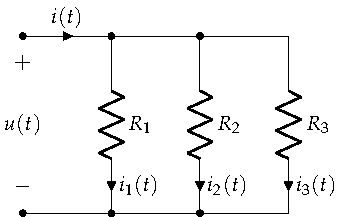
\includegraphics[width=\linewidth]{../figs/AsociacionParalelo.pdf}
\end{center}
\end{column}
\begin{column}{0.33\columnwidth}
\begin{align*}
  u(t) &= \frac{i(t)}{G_1 + G_2 + G_3}\\
  i_3(t) &= G_3 \cdot u(t)\\
  i_3(t)& = i(t) \, \frac{G_3}{G_1 + G_2 + G_3}  
\end{align*}

En general:
\begin{equation*}
  \boxed{i_o(t) = i(t) \cdot \frac{G_o}{G_{eq}}}
\end{equation*}
\end{column}
\begin{column}{0.33\columnwidth}

\begin{align*}
  u(t) &= \frac{i(t)}{\frac{1}{R_1}+\frac{1}{R_2}+\frac{1}{R_3}}\\
  i_3(t) &= \frac{u(t)}{R_3} \\
  i_3(t) &= \frac{i(t)}{R_3} \, \left[\dfrac{1}{ \frac{1}{R_1}+\frac{1}{R_2}+\frac{1}{R_3}}  \right]
\end{align*}

En general:
\begin{equation*}
  \boxed{i_o(t) = i(t)\cdot \frac{R_{eq}}{R_o}}
\end{equation*}
\end{column}
\end{columns}
\end{frame}

\begin{frame}{Conexión en paralelo}{Bobinas}
\begin{columns}
\begin{column}{0.4\columnwidth}
\begin{center}
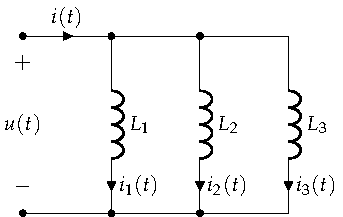
\includegraphics[width=.9\linewidth]{../figs/BobinasParalelo.pdf}
\end{center}
\end{column}
\begin{column}{0.6\columnwidth}
\begin{align*}
  i(t)& = i_1(t) + i_2(t) + i_3(t)\\
  u(t) &= L_1 \cdot \frac{di_1(t)}{dt}= L_2 \cdot \frac{di_2(t)}{dt}= L_3 \cdot \frac{di_3(t)}{dt}\\
  i_1(t)&=\dfrac{1}{L_1}\cdot\int_{0}^{t} u(t)\, dt\\
  i_2(t)&=\dfrac{1}{L_2}\cdot\int_{0}^{t} u(t)\, dt\\
  i_3(t)&=\dfrac{1}{L_3}\cdot\int_{0}^{t} u(t)\, dt\\
  i(t)& = \int u(t)\,dt \cdot \left(\dfrac{1}{L_1}+\dfrac{1}{L_2}+\dfrac{1}{L_3}\right)\\
  \Aboxed{\frac{1}{L_{eq}} &= \sum_{i = 1}^n \frac{1}{L_i}}
\end{align*}
\end{column}
\end{columns}
\end{frame}

\begin{frame}{Conexión en paralelo}{Condensadores}
\begin{columns}
\begin{column}{0.4\columnwidth}
\begin{center}
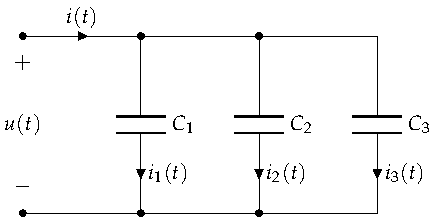
\includegraphics[width=.9\linewidth]{../figs/CondensadoresParalelo.pdf}
\end{center}
\end{column}
\begin{column}{0.6\columnwidth}
\begin{align*}
  i(t) & = i_1(t) + i_2(t) + i_3(t)\\
  i_1(t) &= C_1 \cdot \frac{du(t)}{dt}\\
  i_2(t) &= C_2 \cdot \frac{du(t)}{dt}\\
  i_3(t) &= C_3 \cdot \frac{du(t)}{dt}\\
  i(t)& = \frac{du(t)}{dt} \cdot (C_1 + C_2 + C_3)\\
  \Aboxed{C_{eq} &= \sum_{i = 1}^n C_i}
\end{align*}
\end{column}
\end{columns}
\end{frame}

\begin{frame}{Conexión mixta}{Ejemplo}
    Calcular la corriente que pasa por la fuente de tensión de la figura.
		\begin{figure}[H]
			\centering
			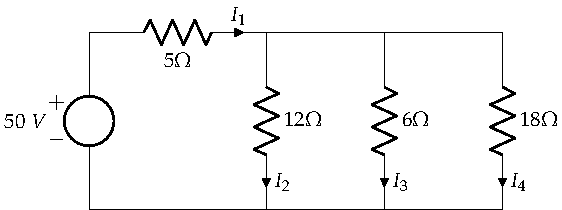
\includegraphics{../figs/ej1_BT1.pdf}
		\end{figure}
\end{frame}

\subsection{Conexión estrella - triángulo}

\begin{frame}{Conexión estrella - triángulo}
\begin{columns}
\begin{column}{0.5\columnwidth}
\begin{center}
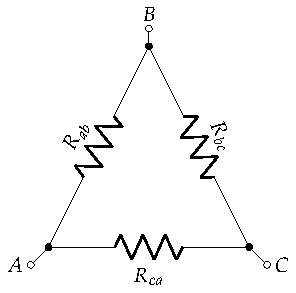
\includegraphics[width=.9\linewidth]{../figs/Conexion_Triangulo.pdf}
\end{center}
\end{column}
\begin{column}{0.5\columnwidth}
\begin{center}
\includegraphics[width=.9\linewidth]{../figs/Conexion_Estrella.pdf}
\end{center}
\end{column}
\end{columns}
\end{frame}

\begin{frame}
{Conexión estrella - triángulo}{Triángulo}
\begin{columns}
\begin{column}{0.5\columnwidth}
\begin{center}
\includegraphics[width=.9\linewidth]{../figs/Conexion_Triangulo.pdf}
\end{center}
\end{column}
\begin{column}{0.5\columnwidth}
\begin{align*}
  R_{AB} &= \frac{R_{ab} \cdot (R_{bc} + R_{ca})}{R_{ab} + R_{bc} + R_{ca}}\\
  \\
  R_{BC} &= \frac{R_{bc} \cdot (R_{ab} + R_{ca})}{R_{ab} + R_{bc} + R_{ca}}\\
  \\
  R_{CA} &= \frac{R_{ca} \cdot (R_{ab} + R_{bc})}{R_{ab} + R_{bc} + R_{ca}}
\end{align*}
\end{column}
\end{columns}
\end{frame}

\begin{frame}{Conexión estrella - triángulo}{Triángulo}
\begin{columns}
\begin{column}{0.5\columnwidth}
\begin{center}
\includegraphics[width=.9\linewidth]{../figs/Conexion_Triangulo.pdf}
\end{center}
\end{column}
\begin{column}{0.5\columnwidth}
\begin{align*}
  R_{AB} &= \frac{R_{ab} \cdot R_{bc}}{R_{ab} + R_{bc} + R_{ca}} + \frac{R_{ab} \cdot R_{ca}}{R_{ab} + R_{bc} + R_{ca}}\\
  \\
  R_{BC} &= \frac{R_{bc} \cdot R_{ab}}{R_{ab} + R_{bc} + R_{ca}} + \frac{R_{bc} \cdot R_{ca}}{R_{ab} + R_{bc} + R_{ca}}\\
  \\
  R_{CA} &= \frac{R_{ca} \cdot R_{ab}}{R_{ab} + R_{bc} + R_{ca}} + \frac{R_{ca} \cdot R_{bc}}{R_{ab} + R_{bc} + R_{ca}}
\end{align*}
\end{column}
\end{columns}
\end{frame}

\begin{frame}{Conexión estrella - triángulo}{Estrella}
\begin{columns}
\begin{column}{0.5\columnwidth}
\begin{center}
\includegraphics[width=.9\linewidth]{../figs/Conexion_Estrella.pdf}
\end{center}
\end{column}
\begin{column}{0.5\columnwidth}
\begin{align*}
  R_{AB} &= R_a + R_b\\
  \\
  R_{BC} &= R_b + R_c\\
  \\
  R_{CA} &= R_c + R_a\\
\end{align*}
\end{column}
\end{columns}
\end{frame}

\begin{frame}{Conexión estrella - triángulo}{Equivalencia}
\begin{align*}
  \frac{R_{a{\color{magenta}b}} \cdot R_{{\color{magenta}b}c}}{R_{ab} + R_{bc} + R_{ca}} + \frac{R_{{\color{teal}a}b} \cdot R_{c{\color{teal}a}}}{R_{ab} + R_{bc} + R_{ca}} &= R_{\color{teal}a} + R_{\color{magenta}b}\\
  \\
  \frac{R_{a{\color{magenta}b}} \cdot R_{{\color{magenta}b}c}}{R_{ab} + R_{bc} + R_{ca}} + \frac{R_{b{\color{orange}c}} \cdot R_{{\color{orange}c}a}}{R_{ab} + R_{bc} + R_{ca}} &= R_{\color{magenta}b} + R_{\color{orange}c}\\
  \\
  \frac{R_{{\color{teal}a}b} \cdot R_{c{\color{teal}a}}}{R_{ab} + R_{bc} + R_{ca}} + \frac{R_{b{\color{orange}c}} \cdot R_{{\color{orange}c}a}}{R_{ab} + R_{bc} + R_{ca}} &= R_{\color{orange}c} + R_{\color{teal}a}
\end{align*}
\end{frame}

\begin{frame}{Conexión estrella - triángulo}{Conversión de triángulo a estrella}
\begin{columns}
\begin{column}{0.3\columnwidth}
\begin{center}
\includegraphics[width=.9\linewidth]{../figs/Conexion_Triangulo.pdf}
\end{center}
\end{column}
\begin{column}{0.4\columnwidth}
\begin{align*}
  R_{\color{teal}a} &= \frac{R_{{\color{teal}a}b} \cdot R_{c\color{teal}a}}{R_{ab} + R_{bc} + R_{ca}}\\
  \\
  R_{\color{magenta}b} &= \frac{R_{a{\color{magenta}b}} \cdot R_{{\color{magenta}b}c}}{R_{ab} + R_{bc} + R_{ca}}\\
  \\
  R_{\color{orange}c} &= \frac{R_{b{\color{orange}c}} \cdot R_{{\color{orange}c}a}}{R_{ab} + R_{bc} + R_{ca}}
\end{align*}
\end{column}

\begin{column}{0.3\columnwidth}
\begin{center}
\includegraphics[width=.9\linewidth]{../figs/Conexion_Estrella.pdf}
\end{center}
\end{column}
\end{columns}
\end{frame}

\begin{frame}
{Conexión estrella - triángulo}{Conversión de estrella a triángulo}
\begin{columns}
\begin{column}{0.3\columnwidth}
\begin{center}
\includegraphics[width=.9\linewidth]{../figs/Conexion_Estrella.pdf}
\end{center}
\end{column}
\begin{column}{0.4\columnwidth}
\begin{align*}
  G_{{\color{teal}a}{\color{magenta}b}} &= \frac{G_{\color{teal}a} \cdot G_{\color{magenta}b}}{G_a + G_b + G_c}\\
  \\
  G_{{\color{magenta}b}{\color{orange}c}} &= \frac{G_{\color{magenta}b} \cdot G_{\color{orange}c}}{G_a + G_b + G_c}\\
  \\
  G_{{\color{orange}c}{\color{teal}a}} &= \frac{G_{\color{orange}c} \cdot G_{\color{teal}a}}{G_a + G_b + G_c}
\end{align*}
\end{column}
\begin{column}{0.3\columnwidth}
\begin{center}
\includegraphics[width=.9\linewidth]{../figs/Conexion_Triangulo.pdf}
\end{center}
\end{column}
\end{columns}
\end{frame}

\begin{frame}{Conexión estrella - triángulo}{Conversión si $R_a=R_b=R_c=R_Y$ y $R_{ab}=R_{bc}=R_{ca}=R_D$}
    
    En el caso concreto de que las resistencias de la estrella/triángulo sean \alert{iguales}\ldots{}
\begin{align*}
  &R_a=R_b=R_c=R_Y\\
  & R_{ab}=R_{bc}=R_{ca}=R_D
\end{align*}
\ldots{} la expresión es:
\begin{equation*}
  \boxed{R_{D} = 3\cdot R_Y}
\end{equation*}
\end{frame}

\begin{frame}{Conexión estrella - triángulo}{Ejemplo}
    Convertir los circuitos de la figura en triángulo o estrella equivalente, según corresponda. 
 \begin{figure}[H]
 		\centering
\includegraphics{../figs/ej7_BT1.pdf}
 	\end{figure}
\end{frame}

\section{Métodos de análisis}

\begin{frame}
\begin{center}
\includegraphics[height=0.95\textheight]{../figs/mallas1.pdf}
\end{center}
\end{frame}

\begin{frame}{Aplicar 1LK}
\begin{columns}
\begin{column}{0.5\columnwidth}
\begin{center}
\includegraphics[width=.9\linewidth]{../figs/mallas1.pdf}
\end{center}
\end{column}

\begin{column}{0.5\columnwidth}
Nudo A
\begin{equation*}
  I_6 = I_1 + I_2
\end{equation*}

Nudo B
\begin{equation*}
  I_1 + I_3 + I_5 = 0
\end{equation*}

Nudo C
\begin{equation*}
  I_2 = I_3 + I_4
\end{equation*}

Nudo D
\begin{equation*}
  I_4 = I_5 + I_6
\end{equation*}
\end{column}
\end{columns}

\vspace{5pt}


No son ecuaciones linealmente independientes:
\begin{equation*}
  C = A + B + D
\end{equation*}
\alert{El número de ecuaciones linealmente independientes aplicando 1LK son $N-1$}
\end{frame}

\begin{frame}{Aplicar 2LK}
\begin{columns}
\begin{column}{0.5\columnwidth}
\begin{center}
\includegraphics[width=.9\linewidth]{../figs/mallas1.pdf}
\end{center}
\end{column}

\begin{column}{0.5\columnwidth}
Malla ABCA
\begin{equation*}
  I_1 \cdot R_1 - \epsilon_1 + \epsilon_2 - I_3 \cdot R_3 - I_2 \cdot R_2 = 0
\end{equation*}

Malla BDCB
\begin{equation*}
  -I_5 \cdot R_5 - I_4 \cdot R_4 + I_3 \cdot R_3 - \epsilon_2 = 0
\end{equation*}

Malla ACDA
\begin{equation*}
  I_2 \cdot R_2 + I_4 \cdot R_4 + I_6 \cdot R_6 - \epsilon_3 = 0
\end{equation*}
\end{column}
\end{columns}

\alert{El número de ecuaciones linealmente independientes aplicando 2LK son $R-N+1$}
\end{frame}

\begin{frame}{Combinar las ecuaciones}
\begin{columns}
\begin{column}{0.5\columnwidth}
\begin{center}
\includegraphics[width=.9\linewidth]{../figs/mallas1.pdf}
\end{center}
\end{column}

\begin{column}{0.5\columnwidth}
\begin{align*}
  - I_1 -  I_2 + I_6  &= 0\\
  I_1 + I_3 + I_5 &= 0\\
  I_4 - I_5 - I_6 &= 0\\
  I_1 \cdot R_1 - I_2 \cdot R_2 - I_3 \cdot R_3 &= \epsilon_1 - \epsilon_2\\
  I_3 \cdot R_3 - I_4 \cdot R_4 -I_5 \cdot R_5 &= \epsilon_2\\
  I_2 \cdot R_2 + I_4 \cdot R_4 + I_6 \cdot R_6 &= \epsilon_3
\end{align*}
\end{column}
\end{columns}
\end{frame}

\begin{frame}{Y en forma matricial}
\begin{equation*}
  \begin{bmatrix}
    -1 & -1 & 0 & 0 & 0 & 1\\
    1 & 0 & 1 & 0 & 1 & 0\\
    0 & 0 & 0 & 1 & -1 & -1\\
    R_1 & -R_2 & - R_3 & 0 & 0 & 0\\
    0 & 0 & R_3 & - R_4 & - R_5 & 0\\
    0 & R_2 & 0 & R_4 & 0 & R_6
  \end{bmatrix} \cdot %
  \begin{bmatrix}
    I_1\\
    I_2\\
    I_3\\
    I_4\\
    I_5\\
    I_6    
  \end{bmatrix} = %
  \begin{bmatrix}
    0\\
    0\\
    0\\
    \epsilon_1 - \epsilon_2\\
    \epsilon_2\\
    \epsilon_3
  \end{bmatrix}
\end{equation*}

Resolver el circuito implica resolver un sistema lineal de \alert{6 ecuaciones}, en el que las incógnitas son las corrientes de cada rama
\end{frame}

\subsection{Método de las mallas}

\begin{frame}{Método de las mallas}
El método de las mallas simplifica el sistema de ecuaciones necesario mediante unas corrientes \emph{ficticias} denominadas \alert{corrientes de malla}, aprovechando las relaciones entre tensiones de la 2LK

\begin{center}
\includegraphics[height=0.7\textheight]{../figs/mallas1_corrientes.pdf}
\end{center}
\end{frame}

\begin{frame}{Método de las mallas}{Relaciones entre las corrientes de rama y malla}
\begin{columns}
\begin{column}{0.6\columnwidth}
\begin{center}
\includegraphics[width=.9\linewidth]{../figs/mallas1_corrientes.pdf}
\end{center}
\end{column}
\begin{column}{0.4\columnwidth}

\begin{align*}
  I_1 &= I_a\\
  I_5 &= -I_b\\
  I_6 &= I_c\\
  I_2 &= I_c -I_a\\
  I_3 &= I_b - I_a\\
  I_4 &= I_c - I_b
\end{align*}
\end{column}
\end{columns}
\end{frame}

\begin{frame}{Método de las mallas}{Aplicar 2LK}
\begin{columns}
\begin{column}{0.4\columnwidth}
\begin{center}
\includegraphics[height=0.45\textheight]{../figs/mallas1_corrientes.pdf}
\end{center}
\end{column}
\begin{column}{0.6\linewidth}
Malla ABCA ($I_a$)
\begin{align*}
  &I_a \cdot R_1 - \epsilon_1 + \epsilon_2 + (I_a - I_b) \cdot R_3 + (I_a - I_c) \cdot R_2 = 0\\
  &I_a \cdot (R_1 + R_3 + R_2)  - I_b\cdot R_3 - I_c \cdot R_2 = \epsilon_1 - \epsilon_2
\end{align*}
Malla BDCB ($I_b$)
\begin{align*}
 & I_b \cdot R_5 + (I_b - I_c) \cdot R_4 + (I_b - I_a) \cdot R_3 - \epsilon_2 = 0\\
&  - I_a \cdot R_3 + I_b \cdot (R_5 + R_4 + R_3) - I_c \cdot R_4 =  \epsilon_2
\end{align*}
Malla ACDA ($I_c$)
\begin{align*}
  &(I_c - I_a) \cdot R_2 + (I_c - I_b) \cdot R_4 + I_c \cdot R_6 - \epsilon_3 = 0\\
  &- I_a \cdot R_2 - I_b \cdot R_4 + I_c \cdot (R_2 + R_4 + R_6) = \epsilon_3
\end{align*}
\end{column}
\end{columns}
\end{frame}


\begin{frame}{Método de las mallas}{En forma matricial}
\begin{center}
\includegraphics[height=0.5\textheight]{../figs/mallas1_corrientes.pdf}
\end{center}
\begin{equation*}
  \begin{bmatrix}
    (R_1 + R_3 + R_2) &  - R_3 & - R_2 \\
    - R_3 & (R_5 + R_4 + R_3) & - R_4 \\
    - R_2 & - R_4 &  (R_2 + R_4 + R_6)
  \end{bmatrix} \cdot %
  \begin{bmatrix}
    I_a\\
    I_b\\
    I_c\\
  \end{bmatrix} = %
  \begin{bmatrix}
    \epsilon_1 - \epsilon_2\\
    \epsilon_2\\
    \epsilon_3
  \end{bmatrix}
\end{equation*}
\end{frame}

\begin{frame}{Método de las mallas}{Ecuación general en forma matricial}
\begin{equation*}
		\begin{bmatrix}
			{\color{magenta}\sum R_{11}} &  {\color{teal}\pm\sum R_{12}} & {\color{teal}{\dots}} & {\color{teal}\pm\sum R_{1n}} \\
			{\color{teal}\pm\sum R_{21}} & {\color{magenta}\sum R_{22}} & {{\dots}} & {\color{teal}\pm\sum R_{2n}} \\
			{\vdots} & {\vdots} &  {\ddots} & \vdots\\
			{\color{teal}\pm\sum R_{n1}} & {\color{teal}\pm\sum R_{n2}} & \dots & {\color{magenta}\sum R_{nn}}
		\end{bmatrix} \cdot 
		\begin{bmatrix}
			I_1\\
			I_2\\
			\vdots\\
			I_n
		\end{bmatrix} = %
		\begin{bmatrix}
			{\color{orange}\sum\epsilon_1}\\
			{\color{orange}\sum\epsilon_2}\\
			{\color{orange}\vdots}\\
			{\color{orange}\sum\epsilon_n}
		\end{bmatrix}
	\end{equation*}
\begin{description}
\item[{\({\color{magenta}\sum R_{ii}}\)}] suma de las resistencias incluidas en la malla de \(I_i\)
\item[{\({\color{teal}\sum R_{ij}}\)}] suma de las resistencias incluidas en las ramas compartidas por las mallas de \(I_i\) e \(I_j\) ($+$ si las corrientes van en el mismo sentido, $-$ en caso contrario)
\item[{\({\color{orange}\sum \epsilon_i}\)}] suma algebraica de las fuerzas electromotrices de los generadores de la malla de \(I_i\) ($+$ si $I_i$ sale por $+$ de la fuente, $-$ en caso contrario)
\end{description}
\end{frame}

\begin{frame}{Método de las mallas}{Procedimiento}
\begin{enumerate}
\item Identificar las corrientes de rama
\item Asignar un sentido a las corrientes de malla
\item Relacionar corrientes de rama con corrientes de malla
\item Escribir ecuación de mallas
\item Resolver la ecuación, obteniendo las corrientes de malla
\item Obtener las corrientes de rama con las relaciones del punto 3
\end{enumerate}

\alert{Importante}: todos los generadores deben ser fuentes de tensión
\end{frame}

\begin{frame}{Método de las mallas}{Ejemplo}
    Calcular las tres intensidades de malla del circuito de la figura.
		\begin{figure}[H]
			\centering
			\includegraphics[]{../figs/ej5_BT1.pdf}
		\end{figure}
\end{frame}

\begin{frame}{Método de las mallas}{Ejemplo}
    Calcular la corriente $I$ en el circuito de la figura.
	    \begin{figure}[H]
	        \centering
	        \includegraphics{../figs/ejemplo_mallas_dependiente.pdf}
	    \end{figure}
\end{frame}

\subsection{Método de los nudos}

\begin{frame}{Método de los nudos}
El método de los nudos aprovecha las relaciones entre corrientes de la 1LK
\begin{center}
\includegraphics[width=.7\linewidth]{../figs/nudos.pdf}
\end{center}
\end{frame}

\begin{frame}{Método de los nudos}{Aplicar 1LK}
\begin{center}
\includegraphics[width=.7\linewidth]{../figs/nudos.pdf}
\end{center}

Nudo A
\begin{equation*}
  I_{g1} - I_a - I_{ab} = 0
\end{equation*}

Nudo B
\begin{equation*}
  I_{ab} - I_{g2} - I_b = 0
\end{equation*}
\end{frame}

\begin{frame}{Método de los nudos}{Tensiones en las resistencias}
\begin{center}
\includegraphics[width=.7\linewidth]{../figs/nudos.pdf}
\end{center}
\begin{align*}
  V_A &= I_a \cdot R_1\rightarrow I_a = \frac{V_A}{R_1}\\
  V_B &= I_b \cdot R_3\rightarrow I_b = \frac{V_B}{R_3}\\
  V_{AB} &= I_{ab} \cdot R_2 \rightarrow I_{ab} = \frac{V_A-V_B}{R_2}
\end{align*}
\end{frame}

\begin{frame}{Método de los nudos}{Combinar las ecuaciones}
\begin{center}
\includegraphics[width=.7\linewidth]{../figs/nudos.pdf}
\end{center}

Nudo A
\begin{equation*}
  I_{g1} - \dfrac{V_A}{R_1} - \dfrac{V_A - V_B}{R_2} = 0 \rightarrow I_{g1} = V_A\cdot\left(\dfrac{1}{R_1}+\dfrac{1}{R_2}\right) - \dfrac{V_B}{R_2} 
\end{equation*}

Nudo B
\begin{equation*}
  \dfrac{V_A - V_B}{R_2} - I_{g2} - \dfrac{V_B}{R_3} = 0 \rightarrow - I_{g2} = - \dfrac{V_A}{R_2} + V_B \cdot\left(\dfrac{1}{R_2} + \dfrac{1}{R_3}\right)
\end{equation*}
\end{frame}

\begin{frame}{Método de los nudos}{Expresión matricial}
\begin{center}
\includegraphics[width=.7\linewidth]{../figs/nudos.pdf}
\end{center}
\begin{equation*}
  \begin{bmatrix}
    \dfrac{1}{R_1}+\dfrac{1}{R_2} & - \dfrac{1}{R_2}\\
    -\dfrac{1}{R_2} & \dfrac{1}{R_2}+\dfrac{1}{R_3}
  \end{bmatrix} \cdot%
  \begin{bmatrix}
    V_A\\
    V_B
  \end{bmatrix} = %
  \begin{bmatrix}
    I_{g1}\\
    -I_{g2}
  \end{bmatrix}
\end{equation*}
\end{frame}

\begin{frame}{Método de los nudos}{Ecuación general}
\begin{equation*}
		\begin{bmatrix}
			{\color{magenta}\sum G_{1}} &  {\color{teal}-\sum G_{12}} & {\color{teal}{\dots}} & {\color{teal}-\sum G_{1n}} \\
			{\color{teal}-\sum G_{21}} & {\color{magenta}\sum G_{2}} & {{\dots}} & {\color{teal}-\sum G_{2n}} \\
			{\vdots} & {\vdots} &  {\ddots} & \vdots\\
			{\color{teal}-\sum G_{n1}} & {\color{teal}-\sum G_{n2}} & \dots & {\color{magenta}\sum G_{n}}
		\end{bmatrix} \cdot 
		\begin{bmatrix}
			U_1\\
			U_2\\
			\vdots\\
			U_n
		\end{bmatrix} = %
		\begin{bmatrix}
			{\color{orange}\sum I_{g1}}\\
			{\color{orange}\sum I_{g2}}\\
			{\color{orange}\vdots}\\
			{\color{orange}\sum I_{gn}}
		\end{bmatrix}
	\end{equation*}

\begin{description}
\item[{\({\color{magenta}\sum G_i}\)}] Suma de las conductancias conectadas al nudo \(i\)
\item[{\({\color{teal}\sum G_{ij}}\)}] Suma de las conductancias conectadas entre los nudos \(i\) y \(j\)
\item[{\({\color{orange}\sum I_{gi}}\)}] Suma algebraica de las corrientes de los generadores conectados en el nudo $i$ ($+$ si entra al nudo, $-$ en caso contrario)
\end{description}

\alert{Importante}: todos los generadores deben ser fuentes de corriente
\end{frame}

\begin{frame}{Método de los nudos}{Ejemplo}
\begin{minipage}[c]{0.5\linewidth}
Determinar las tensiones en los nudos A y B
\begin{align*}
    &\epsilon_1=\qty{6}{\volt}\\
    &\epsilon_2=\qty{12}{\volt} \\
    &\epsilon_3=\qty{24}{\volt}\\
    &I_{g1}= \qty{15}{\ampere}\\
    &I_{g2} =\qty{9}{\ampere}\\
    &I_{g3}= \qty{6}{\ampere}\\
    &R_{1}= R_3 = R_4 = R_5 = \qty{2}{\ohm}\\
    &R_{2}= \qty{1}{\ohm}
\end{align*}
\end{minipage}
\hfill
\begin{minipage}[c]{0.485\linewidth}
\begin{center}
    \includegraphics[width=\linewidth]{../figs/nudos_fuentes.pdf}
\end{center}
\end{minipage}
\end{frame}

\begin{frame}{Método de los nudos modificados}

En el circuito puede haber \alert{fuentes de tensión y de corriente}:
	\begin{enumerate}
	    \item Se supone que, en cada nudo independiente, las corrientes \textbf{salen} de él
	    \item Cada nudo debe cumplir con la 1LK: $\sum I=0$
	    \item En cada nudo, aplicar la siguiente expresión:
	    \begin{equation*}
	        I_{i,j}=\dfrac{U_i-U_j+\sum\pm \epsilon_g}{\sum R}
	    \end{equation*}
	    \begin{description}
	    \item[{$I_{i,j}$}] Corriente que va del nudo $i$ al $j$
	    \item[{$U_i$}] Tensión del nudo del que se sale
	    \item[{$U_j$}] Tensión del nudo al que se llega
	    \item[{$\epsilon_g$}] $fem$ de los generadores por los que se pasa ($+$ si $I$ sale por $+$ de la fuente, $-$ en caso contrario
	    \end{description}
	\end{enumerate}
\end{frame}

\begin{frame}{Método de los nudos modificados}{Ejemplo}
\begin{minipage}[c]{0.5\linewidth}
    Determinar las tensiones en los nudos A y B
\begin{align*}
    &\epsilon_1=\qty{6}{\volt}\\
    &\epsilon_2=\qty{12}{\volt} \\
    &\epsilon_3=\qty{24}{\volt}\\
    &I_{g1}= \qty{15}{\ampere}\\
    &I_{g2} =\qty{9}{\ampere}\\
    &I_{g3}= \qty{6}{\ampere}\\
    &R_{1}= R_3 = R_4 = R_5 = \qty{2}{\ohm}\\
    &R_{2}= \qty{1}{\ohm}
\end{align*}
\end{minipage}
\hfill
\begin{minipage}[c]{0.485\linewidth}
\begin{center}
    \includegraphics[width=\linewidth]{../figs/nudos_fuentes.pdf}
\end{center}
\end{minipage}
\end{frame}

\section{Teoremas}

\subsection{Circuitos lineales} 

\begin{frame}{Circuitos lineales}
Un circuito eléctrico es \alert{lineal} si los elementos pasivos y activos que incluye son lineales:
	\begin{itemize}
	    \item \alert{Elemento pasivo}: la relación entre tensión y corriente es lineal ($R$, $L$, $C$)
        \item \alert{Fuente dependiente}: su salida tiene una relación lineal con la magnitud del circuito de la que depende
	\end{itemize}
Propiedades:
\begin{itemize}
    \item \alert{Proporcionalidad}: Sea $y(t)$ la respuesta de un circuito lineal a una excitación $x(t)$. Si la excitación es multiplicada por una constante, $K\cdot x(t)$, la respuesta del circuito será modificada por la misma constante, $K \cdot y(t)$.
    \item \textbf{Superposición}: La respuesta de un circuito lineal a varias fuentes de excitación actuando simultáneamente es igual a la suma de las respuestas que se tendrían cuando actuase cada una de ellas por separado:
    \begin{equation*}
        y(t)=\sum_i y_i(t)
    \end{equation*}
\end{itemize}
    
\end{frame}


\subsection{Teoremas de Thévenin y Norton}

\begin{frame}{Teoremas de Thévenin y Norton}

\begin{itemize}
    \item Interés solo en \alert{una parte} del circuito
    \item Transforman red compleja en una equivalente \alert{más simple}
\end{itemize}

\begin{center}
\includegraphics[width=.4\linewidth]{../figs/thevenin_continua_red.pdf}
\end{center}
\end{frame}

\begin{frame}{Teoremas de Thévenin y Norton}{Thévenin}
    Cualquier \alert{red lineal} compuesta por elementos activos y pasivos puede sustituirse, desde el punto de vista de sus terminales externos AB, por una \alert{fuente de tensión} (generador de Thévenin, \(\epsilon_{th}\)) en \alert{serie} con una resistencia (resistencia de Thévenin, \(R_{th}\)).
    
    \begin{center}
\includegraphics[width=.38\linewidth]{../figs/thevenin_continua.pdf}
\end{center}
\end{frame}

\begin{frame}{Teoremas de Thévenin y Norton}{Cálculo del equivalente de Thévenin}
\begin{minipage}[c]{0.4\linewidth}
\begin{center}
\includegraphics[width=.9\linewidth]{../figs/thevenin_continua.pdf}
\end{center}
\end{minipage}
\hfill
\begin{minipage}[c]{0.58\linewidth}
\begin{itemize}
\item Circuito Abierto (\(R_L \to \infty, \quad U_{AB} = U_{oc}\))
\[
\boxed{\epsilon_{th} = U_{oc}}
\]
\item Cortocircuito (\(R_L = 0, \quad I = I_{sc}\))
\end{itemize}
\[
\boxed{R_{th} = \frac{\epsilon_{th}}{I_{sc}} = \frac{U_{oc}}{I_{sc}}}
\]
\end{minipage}

\vspace{5mm}
\alert{Importante:} Si no hay fuentes dependientes, $R_{th}$ se puede calcular como la \alert{resistencia} equivalente desde los terminales AB (anulando las fuentes independientes)
\end{frame}

\begin{frame}{Teoremas de Thévenin y Norton}{Norton}
Cualquier \alert{red lineal} compuesta por elementos activos y pasivos puede sustituirse, desde el punto de vista de sus terminales externos AB, por una \alert{fuente de corriente} (generador de Norton, \(I_N\)) en \alert{paralelo} con una resistencia (resistencia de Norton, \(R_N\)).

\begin{center}
\includegraphics[width=.37\linewidth]{../figs/norton_continua.pdf}
\end{center}
\end{frame}



\begin{frame}{Teoremas de Thévenin y Norton}{Cálculo del equivalente de Norton}
\begin{minipage}[c]{0.4\linewidth}
\begin{center}
\includegraphics[width=.9\linewidth]{../figs/norton_continua.pdf}
\end{center}
\end{minipage}
\hfill
\begin{minipage}[c]{0.58\linewidth}
\begin{itemize}
\item Cortocircuito (\(R_L = 0, \quad I = I_{sc}\))
\end{itemize}
\[
\boxed{I_N = I_{sc}}
\]
\begin{itemize}
\item Circuito Abierto (\(R_L \to \infty, \quad U_{AB} = U_{oc}\))
\end{itemize}
\[
\boxed{R_N = \frac{U_{oc}}{I_N} = \frac{U_{oc}}{I_{sc}}}
\]
\end{minipage}

\vspace{5mm}
\alert{Importante:} Si no hay fuentes dependientes, $R_{N}$ se puede calcular como la \alert{resistencia} equivalente desde los terminales AB (anulando las fuentes independientes)
\end{frame}

\begin{frame}{Teoremas de Thévenin y Norton}{Ejemplo}
Determinar el equivalente de Thévenin del circuito de la figura visto desde los terminales $A-B$, y la potencia que se disiparía si se conectase una resistencia de 5$\Omega$.
    \begin{figure}[H]
        \centering
        \includegraphics{../figs/ej_Th_cc1.pdf}
    \end{figure}
\end{frame}

\begin{frame}{Teoremas de Thévenin y Norton}{Ejemplo}
    En el circuito de la figura, calcular el equivalente de Norton.

Datos: $R = {1}{\Omega};\; \epsilon_g = {10}{V};\; \alpha = \beta = 1$

\begin{figure}[H]
    \centering
    \includegraphics[width=0.45\linewidth]{../figs/ejemplo_norton.pdf}
\end{figure}
\end{frame}

\subsection{Teorema de la máxima transferencia de potencia}

\begin{frame}{Teorema de la máxima transferencia de potencia}{Planteamiento}
¿Qué resistencia \(R_L\) hay que conectar en los terminales AB para que el circuito entregue la \alert{máxima potencia disponible}?

\begin{center}
\includegraphics[height=0.55\textheight]{../figs/thevenin_continua_red.pdf}
\end{center}

Se aplica el \alert{equivalente de Thévenin}
\end{frame}

\begin{frame}{Teorema de la máxima transferencia de potencia}{Ecuaciones}
Calculamos la potencia activa en la impedancia de carga \(Z_L\):
\begin{columns}
\begin{column}{0.35\columnwidth}
\begin{center}
\includegraphics[height=0.45\textheight]{../figs/thevenin_continua.pdf}
\end{center}
\end{column}


\begin{column}{0.5\columnwidth}
\begin{align*}
{I} &= \frac{{\epsilon}_{th}}{R_{th} + R_L}\\
P_L &= I^2 \cdot R_L\\
\Aboxed{P_L &= \frac{\epsilon^2_{th}}{(R_{th} + R_L)^2} \cdot R_L}
\end{align*}
\end{column}
\end{columns}

La condición de máximo es: 
\[
  \boxed{%
    \diffp{P_L}{R_L} = 0%
  }
\]
\end{frame}

\begin{frame}{Teorema de la máxima transferencia de potencia}{Resistencia}
\begin{equation*}
        \diffp{P_L}{R_L} = \epsilon^2_{th} \cdot \left[\frac{1}{(R_L + R_{th})^2} - 2 \cdot \frac{R_L}{(R_L + R_{th})^3}\right]= \frac{\epsilon^2_{th} \cdot (R_{th} - R_L)}{(R_L + R_{th})^3}
    \end{equation*}
Aplicando la condición de máximo:
\[
   \diffp{P_L}{R_L} = 0 \Rightarrow \boxed{R_L = R_{th}}
\]
\end{frame}

\begin{frame}{Teorema de la máxima transferencia de potencia}{Impedancia de carga}
Dado un circuito lineal (del que se puede calcular su equivalente de Thévenin) \ldots{}
\begin{center}
\includegraphics[height=0.45\textheight]{../figs/thevenin_continua.pdf}
\end{center}

\ldots{} la resistencia de carga que hay que conectar entre sus terminales AB para obtener la máxima potencia disponible es:
\[
  \boxed{R_L = R_{th}}
\]
\end{frame}

\begin{frame}{Teorema de la máxima transferencia de potencia}{Máxima potencia disponible}
La máxima potencia disponible en la carga es:

\vspace{5mm}
\begin{minipage}[c]{0.4\linewidth}
\begin{center}
\includegraphics[height=0.45\textheight]{../figs/thevenin_continua.pdf}
\end{center}
\end{minipage}
\hfill
\begin{minipage}[c]{0.58\linewidth}
\begin{equation*}
  \left.
    \begin{matrix}
      R_L = R_{th}\\
      P_L = \frac{\epsilon^2_{th}}{(R_{th} + R_L)^2} \cdot R_L
    \end{matrix} \right\}\rightarrow
  \boxed{P_L = \frac{\epsilon^2_{th}}{4 R_{th}}}
\end{equation*}

\begin{block}{Importante}
Esta expresión es \alert{válida únicamente} para calcular la máxima transferencia de potencia
\end{block}
\end{minipage}
\end{frame}

\subsection{Teorema de superposición}

\begin{frame}{Teorema de superposición}{Elementos lineales}
Un circuito eléctrico es lineal si los elementos pasivos y activos que incluye son lineales:
\begin{itemize}
\item Un \alert{elemento pasivo} es lineal si la relación entre la tensión entre sus terminales y la corriente que lo recorre es lineal: \alert{resistencias, condensadores y bobinas}.
\item Una \alert{fuente dependiente} es lineal si su salida (tensión o corriente) tiene una relación lineal con la magnitud del circuito de la que depende.
\item Un circuito lineal tiene dos propiedades:
\begin{itemize}
\item Homogeneidad o \alert{proporcionalidad}
\item Aditividad o \alert{superposición}
\end{itemize}
\end{itemize}
\end{frame}

\begin{frame}{Teorema de superposición}%{Aditividad o Superposición}
\begin{columns}
\begin{column}{0.5\columnwidth}
La respuesta de un \alert{circuito lineal} a varias fuentes de excitación actuando simultáneamente es igual a la suma de las respuestas que se tendrían cuando actuase cada una de ellas por separado

\[
y(t) = \sum_i y_i(t)
\]
\end{column}

\begin{column}{0.5\columnwidth}
\begin{center}
\includegraphics[width=\linewidth]{../figs/superposicion.pdf}
\end{center}
\end{column}
\end{columns}
\end{frame}

\begin{frame}{Teorema de superposición}{Análisis de un circuito mediante superposición}
\begin{block}{Procedimiento}
\begin{enumerate}
\item Se apagan todas las fuentes \alert{independientes} del circuito menos una
\begin{itemize}
\item Las fuentes de tensión se sustituyen por un cortocircuito (\(U = 0\))
\item Las fuentes de corriente se sustituyen por un circuito abierto (\(I = 0\))
\item Las fuentes {dependientes} {no} se modifican
\end{itemize}
\item Se analiza el circuito, obteniendo la respuesta individual a la fuente que permanece activa
\item Se repite este procedimiento para cada una de las fuentes \alert{independientes} del circuito
\item La respuesta total del circuito es la suma de las respuestas individuales
\end{enumerate}
\end{block}
\end{frame}

\begin{frame}{Teorema de superposición}{Ejemplo}
    Usar el principio de superposición para encontrar $U_0$ en el circuito de la figura.
    \begin{figure}[H]
        \centering
        \includegraphics[width=0.5\linewidth]{../figs/ej_superposicion_cc.pdf}
    \end{figure}
\end{frame}

\end{document}
